\documentclass[a4paper]{report}

% Setup layout
\usepackage{geometry}
\geometry{paper=a4paper}

% Font setup
\usepackage[T1]{fontenc}
\usepackage[utf8]{inputenx}
\usepackage{palatino}
\usepackage{mathpazo}
\usepackage{microtype}
\renewcommand*\ttdefault{txtt}

% Language setup
\usepackage[czech,english]{babel}

% Setup hyperlinks in PDF
\usepackage[
  pdftex,
  breaklinks=true,
  pdfborder={0 0 0}
]{hyperref}

% Glossaries
\usepackage[sort=def, xindy, nonumberlist]{glossaries}
\usepackage{glossary-long}
\makeglossaries

% Other includes
\usepackage{url}
\usepackage{paralist}
\usepackage{parcolumns}
\usepackage{xcolor}
\usepackage{graphicx}
\usepackage{longtable}
\usepackage{multirow}
\usepackage{tikz}

% If then else
\usepackage{ifthen}

% Code listing
\usepackage{verbatim}
\usepackage{listingsutf8}
\usepackage{showexpl}
\lstset{
  escapechar=\⠶
}

% Bibliography
\usepackage[nottoc]{tocbibind}
\bibliographystyle{elsarticle-num}

% Command \provideenvironment and \providecounter
\makeatletter
\def\provideenvironment{\@star@or@long\provide@environment}
\def\provide@environment#1{%
        \@ifundefined{#1}%
                {\def\reserved@a{\newenvironment{#1}}}%
                {\def\reserved@a{\renewenvironment{dummy@environ}}}%
        \reserved@a
}
\def\dummy@environ{}
\makeatother
\makeatletter
\newcommand*\providecounter[1]{%
  \@ifundefined{c@#1}%
    {\@definecounter{#1}}%
    {}%
}
\makeatother

% Command \todo
\newcommand{\todo}[1]{%
\def\empty{}%
\def\prvniparametr{#1}%
\ifx\prvniparametr\empty%
\begingroup\small\tt\textcolor{red}{\noindent\textbf{TODO}}\endgroup
\else%
\begingroup\small\tt\textcolor{red}{\noindent\textbf{TODO:}\ #1}\endgroup
\fi%
}

% Code inline
\lstdefinestyle{lstStyleShort}{
  breaklines=true,
  breakatwhitespace=true,
  breakautoindent=true,
}
\newcommand{\code}[1]{\textbf{\small\texttt{#1}}}

% Document title page
\author{Petr Holub, Jan Růžička, Miloš Liška, Martin Šrom, Ondřej Pavelka, Ondřej Bouda}
\date{\copyright~CESNET~z.\,s.\,p.\,o.\\2012}

%%%%%%%%%%%%%%%%%%%%%%%%%%%%%%%%%%%%%%%%%%%%%%%%%%%%%%%%%%%%%%%%%%%%%%%%%%%%%%%%
% Entity example (type, name, comment)
\lstnewenvironment{ObjectCode}[3]{%
    \removelastskip
    \vskip 3mm
    \lstset{
      aboveskip=0pt,
      belowskip=0pt,    
      xleftmargin=8pt,
      basicstyle=\fontfamily{txtt}\selectfont,
      keywordstyle=\fontseries{b}\selectfont,
    }
    \minipage{\textwidth}
    \advance\leftmargini -3mm \quote
    \footnotesize\ttfamily #2 = \ifx&#1&\else\textbf{#1} \fi{}\{
    \ifx&#3& \else {\color{gray}// #3} \fi
}{%    
    \vspace*{-4pt}
    \footnotesize\ttfamily \}
    \endquote
    \endminipage
    \vskip 3mm
}




\usepackage{titlesec}

\titleformat{\chapter}[display]
    {\normalfont\LARGE\bfseries}{\chaptertitlename\ \thechapter}{10pt}{\Huge}
\titlespacing*{\chapter}{0pt}{0pt}{20pt}
\titlespacing{\paragraph}{0pt}{0.1\baselineskip}{1em}

\addtolength{\textheight}{100pt}
\setlength{\hoffset}{-25pt}
\setlength{\voffset}{-40pt}
\addtolength{\textwidth}{50pt}


\lstnewenvironment{Entity}{%
    \removelastskip
    \vskip 2mm
    \lstset{
      aboveskip=0pt,
      belowskip=0pt,    
      basicstyle=\fontfamily{txtt}\selectfont,
      keywordstyle=\fontseries{b}\selectfont,
      comment=[l]{//},  
	  morekeywords={
		StandaloneTerminalCapability, RoomProviderCapability, AliasProviderCapability, ValueProvider, PatternValueProvider,
		Alias, Resource, DeviceResource, ManagedMode,
		PeriodicDateTimeSlot, PeriodicDateTime,
		ReservationRequest, ReservationRequestSet, 
		ResourceSpecification, AliasSpecification, RoomSpecification, H323RoomSetting, UserPerson,
		CompartmentSpecification, PersonSpecification, ExistingEndpointSpecification, ExternalEndpointSetSpecification,
		H323, SIP, ADOBE_CONNECT, SCIENCE, H323_E164, SIP_URI, ADOBE_CONNECT_URI
	  }          
    }
    \minipage{\textwidth}    
}{%    
    \vspace*{-4pt}
    \endminipage
    \vskip 3mm
}


\begin{document}

\title{Shongo Architecture}
\maketitle
\tableofcontents




\chapter{Architecture}

Shongo is a reservation system designed for booking videoconferencing resources. It is composed of several components (see fig. \ref{fig:architecture}):

\begin{enumerate}

\item \textbf{Controller} is the main backend application for a single domain written in Java which holds a relational database of resources, reservation requests and all other entities. Controller provides an XML-RPC API which is used by clients to manage the relational database and to control managed devices for the domain. Controller schedules reservations, informs users about theirs reservations by email and executes meetings in devices via connectors.

\item \textbf{Web/Cmd-line Client} is an application written in Perl which allows the users/administrators to access the controller (e.g., to create/modify/delete the resources and reservation requests and to control managed devices).

\item \textbf{Connector} is an application written in Java which runs one or more \textbf{Device Agents} and which mediates the communication to controller via JADE (middle-ware written in Java for creating multi-agent systems)

\item \textbf{Device Agent} is a sub-component of \textbf{Connector} which manages a single videoconferencing device (e.g., Cisco Codian MCU, Adobe Connect server, LifeSize endpoint or Tandberg Codec endpoint). It is able, for instance, to create/modify/delete a room or to dial/hangup a participant in multipoint devices or to dial/hangup on endpoints (and more).

\item \textbf{Auth Server} is a component for user authentication/authorization and for lookuping existing users from identity providers. It is used by \textbf{Web Client} for user sign up and by \textbf{Controller} to verify the user identity and to lookup user information.

\end{enumerate}

\begin{figure}[ht!]
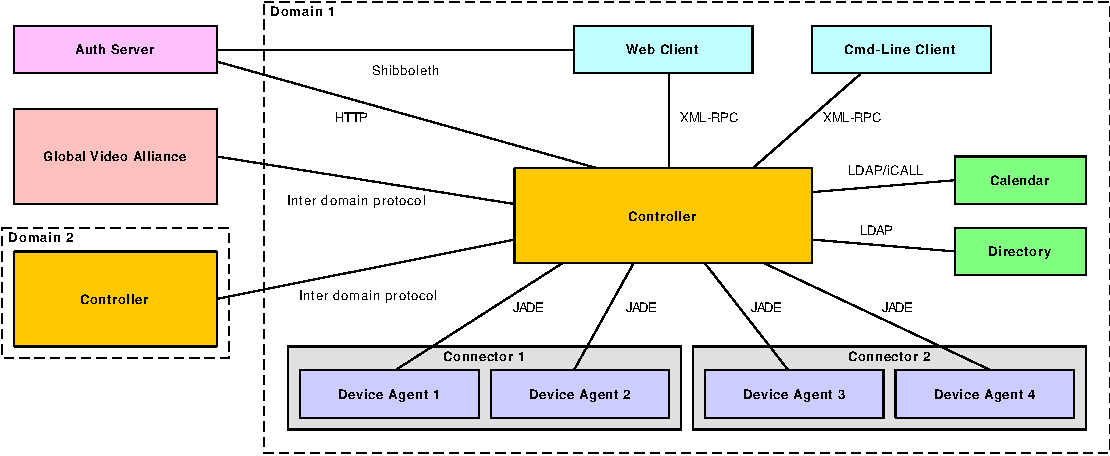
\includegraphics[width=\textwidth]{diagrams/dd_architecture}
\caption{Architecture of Shongo reservation system}
\label{fig:architecture}
\end{figure}

Shongo isn't currently fully implemented. In the current state each Shongo instance is able to manage resources in a single domain without the inter-domain collaboration. The Shongo instance means deployed controller, web client and one or more connectors with one or more device agents. The fig. \ref{fig:architecture-implemented} shows which components and communication channels are already implemented.

\begin{figure}[ht!]
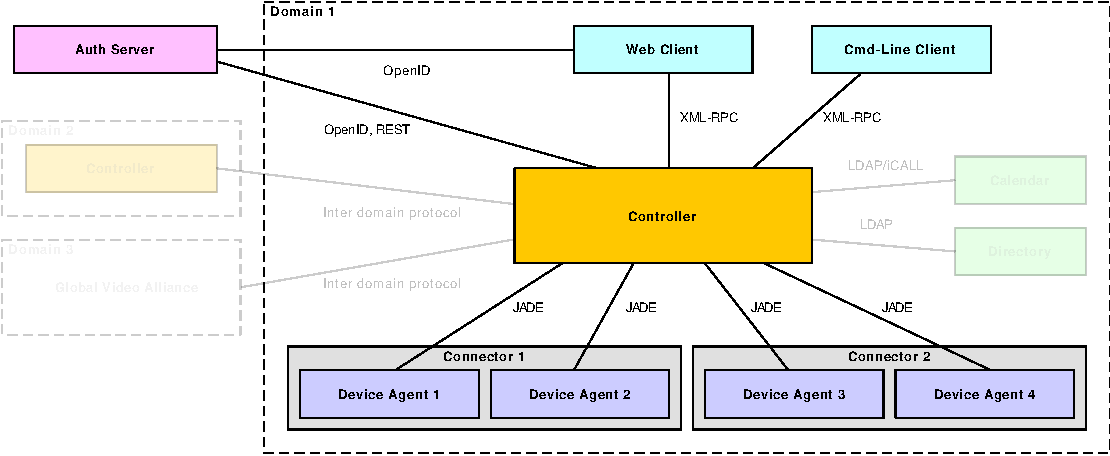
\includegraphics[width=\textwidth]{diagrams/dd_architecture_implemented}
\caption{Already implemented components in Shongo reservation system (grayed parts aren't implemented yet)}
\label{fig:architecture-implemented}
\end{figure}




\chapter{Deployment}

Shongo reservatin system for a single domain can be deployed to target machines in several ways (see fig. \ref{fig:deployment} for examples).

\begin{figure}[ht!]
\begin{center}  
  \subfigure[All components are deployed to the same machine]{
    \label{fig:deployment:one}
    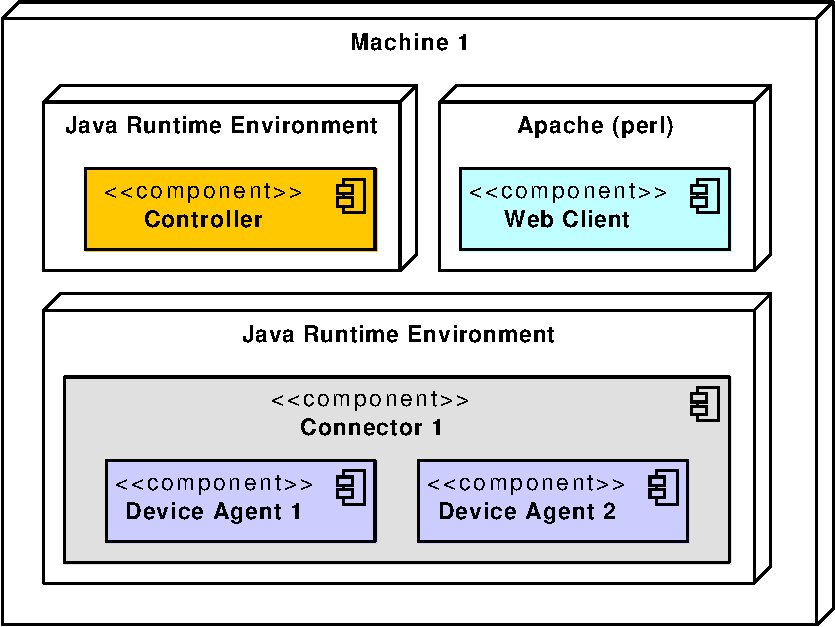
\includegraphics[width=7.5cm]{diagrams/dd_deployment_one}
  } 
  \hfill
  \subfigure[Controller and web client are deployed to the same machine and connector is deployed to another one]{
    \label{fig:deployment:two}
    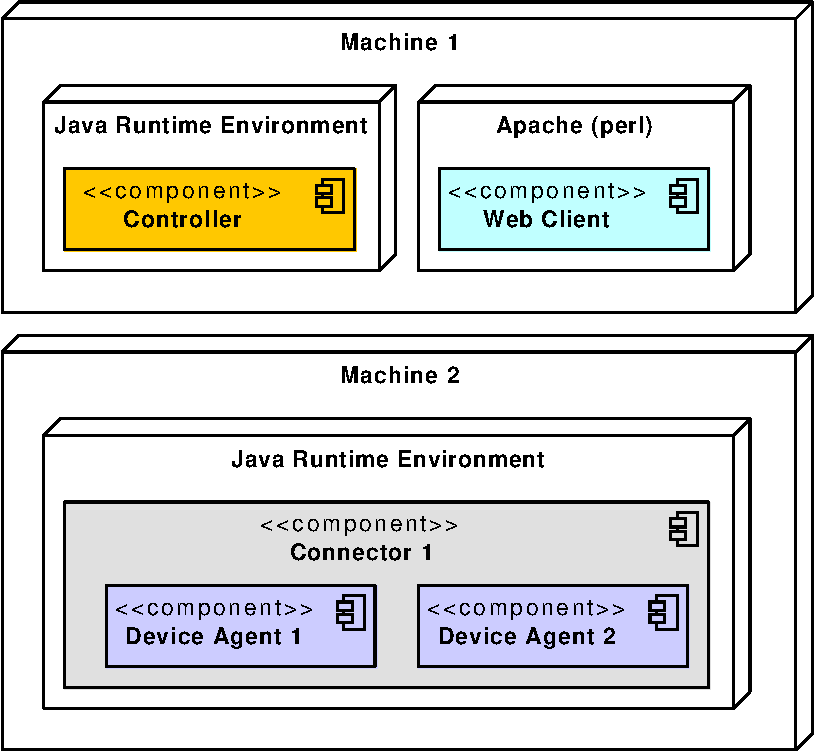
\includegraphics[width=7.5cm]{diagrams/dd_deployment_two}
  } 
  \subfigure[Each component is deployed to it's own machine]{
    \label{fig:deployment:multi}
    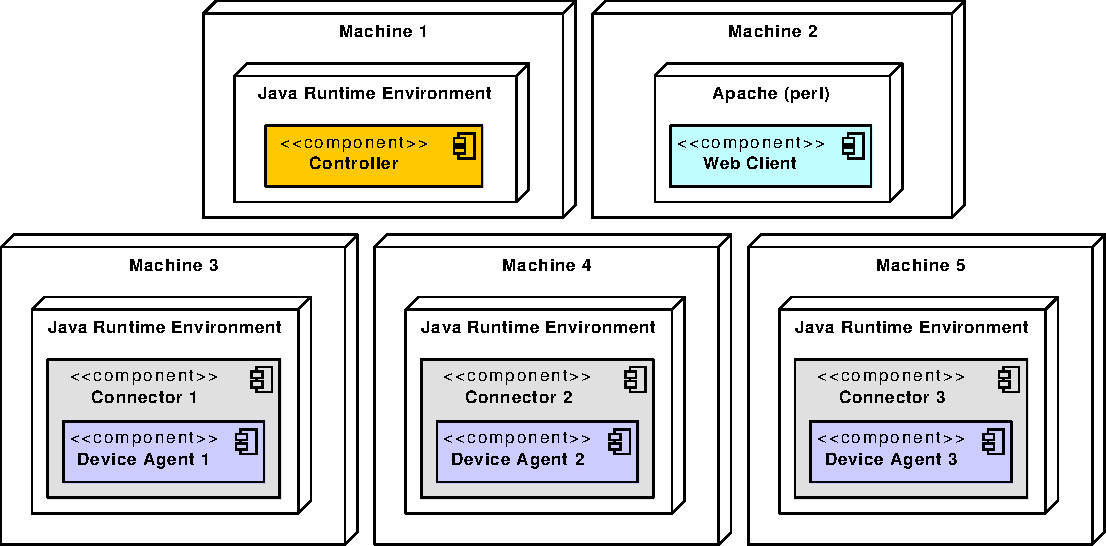
\includegraphics[width=14cm]{diagrams/dd_deployment_multi}
  } 
\end{center}
\caption{Examples of deployment of Shongo reservation system components}
\label{fig:deployment}
\end{figure}




\chapter{Controller}

As it was written in the first chapter, the controller is the main backend application for a single domain. It is a command-line application written in Java which must be started as long as the reservation system for a domain should be in operation.
Controller is composed of several sub-components:

\begin{itemize}

\item \textbf{API} receives and processes user and administrator requests. Basically the API stores some data to database (e.g., resource or reservation request) or immediately performs some action based on the request (e.g., retrieves actual room list from MCU device or determines status of Tandberg endpoint).

\item \textbf{Scheduler} processes complete reservation requests from database and tries to allocate them as reservations. The resulting reservations from scheduler are stored to database. As part of some reservations can be allocated special entities referred to as executables. Executable is an entity which can be started/stopped, e.g., room on MCU, meetting in Adobe Connect, call between two endpoints or compartment which represents a set of multiple interconnected rooms (e.g., two rooms on different MCUs).

\item \textbf{Executor} processes executables from database and tries to start/update/stop them at the right moment (e.g., tries to create a room in MCU device, add new participant to Adobe Connect meeting, stop meeting in Adobe Connect or dial a call between two Tandberg endpoints).

\item \textbf{Authorization} is a sub-component which is used for:
\begin{compactitem} 
\item verifying user identity against the \textbf{Auth Server}. The most of API requests must contain the user identity (OpenID \cite{openid} access token) which is verified.
\item lookuping existing users from identity providers via the \textbf{Auth Server}. 
\item managing ACL rules, i.e., triples \codeValue{(user, entity, role)}, where \codeValue{user} is unique user identifier from \textbf{Auth Server}, \codeValue{entity} is unique identifier of entity in controller database (e.g., resource, reservation request, reservation or executable) and \codeValue{role} is a possible user role for the entity (e.g., \codeValue{owner}).
\end{compactitem}

\end{itemize}

Figure \ref{fig:reservation-request-processing} shows how a reservation request created by an user is processed by the controller.

\begin{figure}[b!]
\centering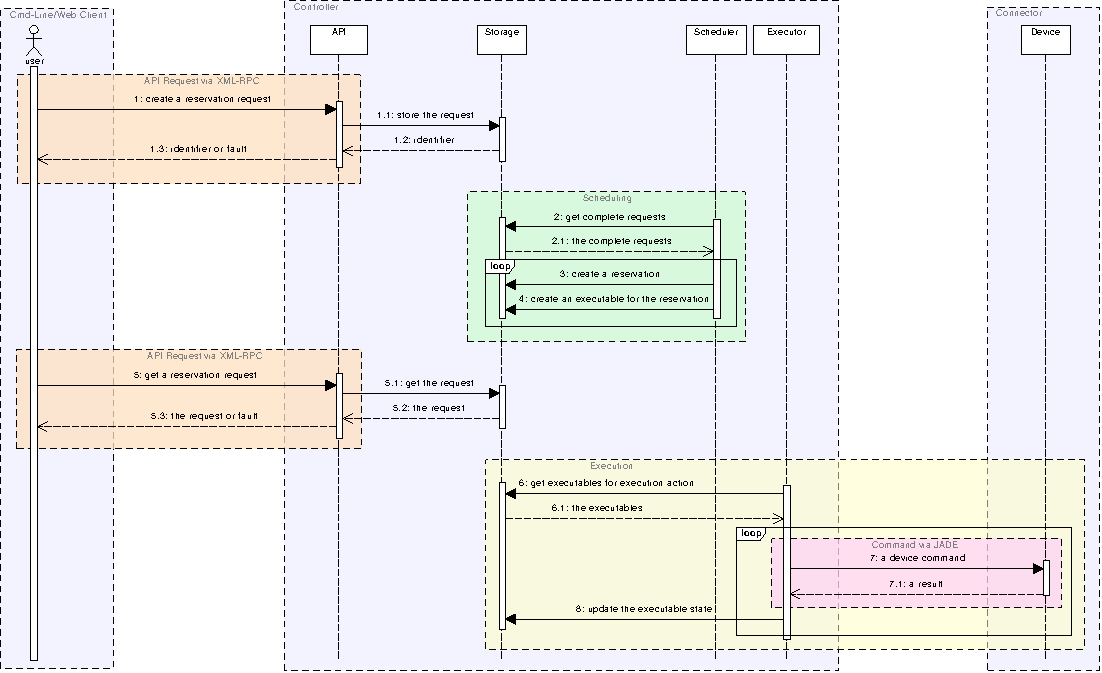
\includegraphics[width=\textwidth]{diagrams/sd_reservation_request_processing}
\caption{Process of creating reservation request by an user, allocating reservation by the scheduler and executing the meeting by the executor}
\label{fig:reservation-request-processing}
\end{figure}
\cleardoublepage




\section{Relational Database}

This section shows the controller relational database schema and few examples of entities which can be stored insided the database.



\subsection{Resources}

\begin{figure}[ht!]
\centering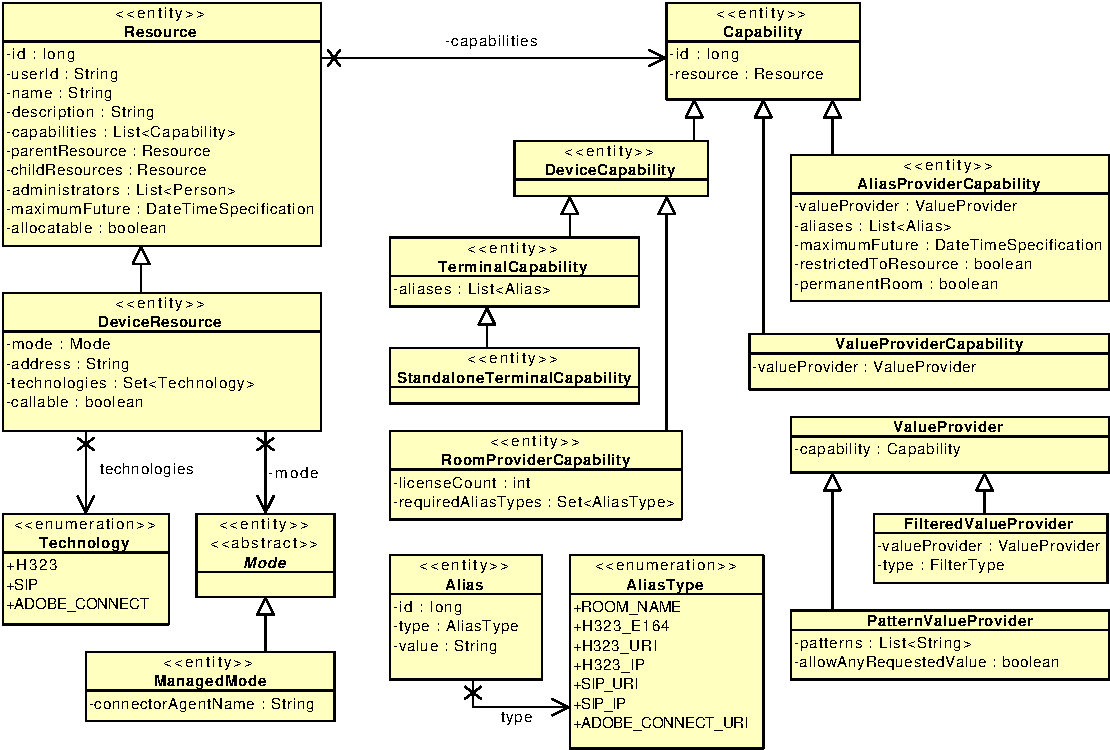
\includegraphics[width=0.9\textwidth]{diagrams/cd_resources}
\caption{Database schema of resources}
\label{fig:resources}
\end{figure}

Examples of resources which can be stored insided the relational database:

\begin{itemize}

\item Hardware endpoint Tandberg Codec C90 which is accessible by H.323 number 950087300 and sip:950087300@cesnet.cz.
\begin{Entity}
DeviceResource {
  name: "Tandberg Codec C90",
  technologies: [H323, SIP],
  capabilities: [
    StandaloneTerminalCapability {
      aliases: [
        Alias { type: H323_E164, value: "950087300"},
        Alias { type: SIP_URI,   value: "sip:950087300@cesnet.cz"},  	  	
      ]
    }
  ] 
}
\end{Entity}

\newpage
\item Cisco Codian MCU which can host multiple H.323 virtual rooms (the limit is 30 participants for all rooms) and which can assign H.323 numbers in range 950087200 - 950087299 to hosted rooms.
\begin{Entity}
DeviceResource {
  id: 1,
  name: "Cisco Codian MCU",
  technologies: [H323, SIP],
  capabilities: [
    RoomProviderCapability {
      licenseCount: 30,
      requiredAliasTypes: [H323_E164]
    },
    AliasProviderCapability {
      valueProvider: PatternValueProvider {
        patterns: "950087{range:200:299}"
      },
      aliases: [Alias { type: H323_E164, value: "{value}"}],
      restrictedToResource: true 
    }
  ]
}
\end{Entity}

\item Adobe Connect server which can host multiple meetings (the limit is 100 participants for all meetings).
\begin{Entity}
DeviceResource {
  id: 2,
  name: "Adobe Connect server",
  address: "connect.cesnet.cz",
  technologies: [ADOBE_CONNECT],
  capabilities: [
    RoomProviderCapability {
      licenseCount: 100,
      requiredAliasTypes: [ADOBE_CONNECT_URI]
    },
    AliasProviderCapability {
      valueProvider: PatternValueProvider {
        patterns: "{hash:6}"
      },
      aliases: [Alias { type: ADOBE_CONNECT_URI, value: "{device.address}/{value}"}],
      restrictedToResource: true 
    }
  ]
}
\end{Entity}

\item Physical conference room.

\begin{Entity}
Resource {
  id: 3,
  name: "Conference Room C300",
}
\end{Entity}

\item And more...

\end{itemize}



\cleardoublepage
\subsection{Reservation Requests}

\begin{figure}[ht!]
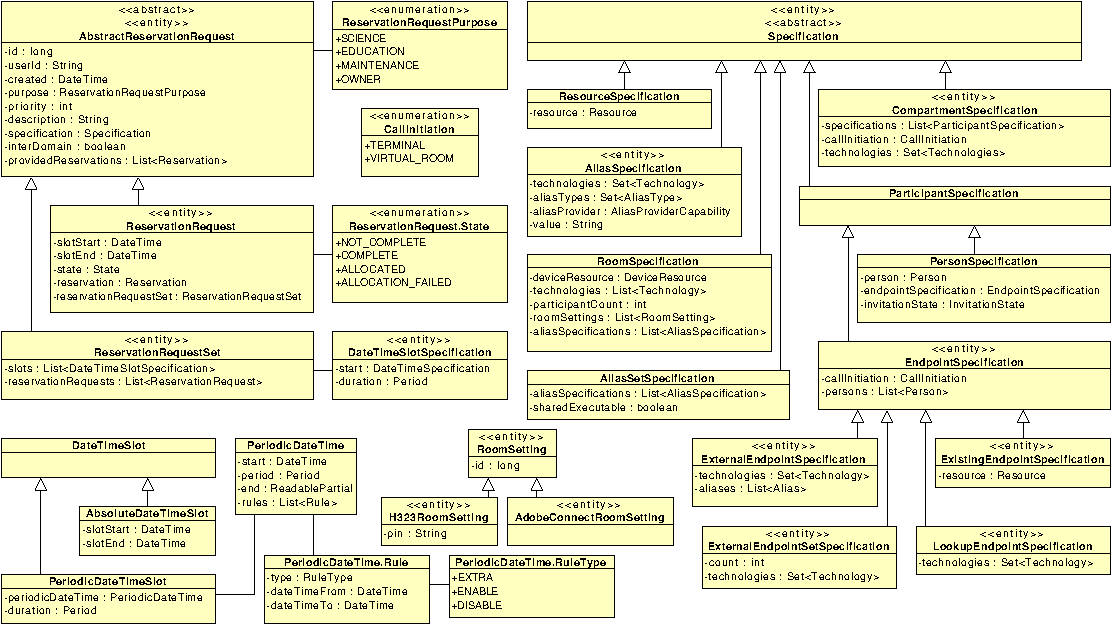
\includegraphics[width=\textwidth]{diagrams/cd_reservation_requests}
\caption{Database schema of reservation requests}
\label{fig:reservation-requests}
\end{figure}

Examples of reservation requests:

\begin{itemize}

\item Request for booking physical conference room from 12:00 to 14:00 on 2013-04-10 UTC.
\begin{Entity}
ReservationRequest {
  slotStart: "2013-04-10T12:00Z",
  slotEnd:   "2013-04-10T14:00Z",
  specification: ResourceSpecification {
    resource: Resource { id: 3 }
  }
}
\end{Entity}

\item Request for booking H.323/SIP room for 5 participants from 12:00 to 14:00 UTC on 2013-04-10. The room will be restricted by PIN code 1234.
\begin{Entity}
ReservationRequest {
  slotStart: "2013-04-10T12:00Z",
  slotEnd:   "2013-04-10T14:00Z",
  specification: RoomSpecification {
    participantCount: 5,
    technologies: [H323, SIP],
    roomSettings: [
      H323RoomSetting { pin: "1234" }
    ]
  }
}
\end{Entity}

\newpage
\item Request for booking H.323/SIP room for 5 participants every Monday from 12:00 to 14:00 UTC in April 2013 with H.323 number 950087250.
\begin{Entity}
ReservationRequestSet {
  slots: [
    PeriodicDateTimeSlot {
      periodicDateTime: PeriodicDateTime {
        start:  "2013-04-10T12:00Z",
        period: "P1W",
        end:    "2013-04-30"
      },
      duration: "PT2H"
    }
  ]
  specification: RoomSpecification {
    participantCount: 5,
    technologies: [H323, SIP]
    aliasSpecifications: [
      AliasSpecification { aliasTypes: [H323_E164], value: "950087250" }
    ]
  }
}
\end{Entity}

\item Request for booking meeting from 12:00 to 14:00 UTC on 2013-04-10. Controller will invite Martin Šrom and Peter Holub by email to attend the meeting and to select which endpoint they will use for connecting. After they accept/reject the invitation, the request become complete and controller can allocate a meeting room (or series of interconnected rooms) for number of accepted participants plus 3 (one existing endpoint plus two H.323/SIP ports for guests). When the meeting starts the controller automatically dials out the Tandberg Codec C90. The invitation of participants and allocation of multiple interconnected rooms is not fully implemented yet.
\begin{Entity}
ReservationRequest {
  slotStart: "2013-04-10T12:00Z",
  slotEnd:   "2013-04-10T14:00Z",
  specification: CompartmentSpecification {
    participantSpecifications: [
      PersonSpecification {
        person: UserPerson { id: "srom@cesnet.cz"}
      },
      PersonSpecification {
        person: UserPerson { id: "holub@cesnet.cz"}
      },      
      ExistingEndpointSpecification { 
        resource: Resource { id: 1 } 
      },
      ExternalEndpointSetSpecification {
        count: 2,
        technologies: [H323, SIP]
      }
    ],    
  }
}
\end{Entity}

\item And more...

\end{itemize}



\cleardoublepage
\subsection{Reservations}

\begin{figure}[ht!]
\centering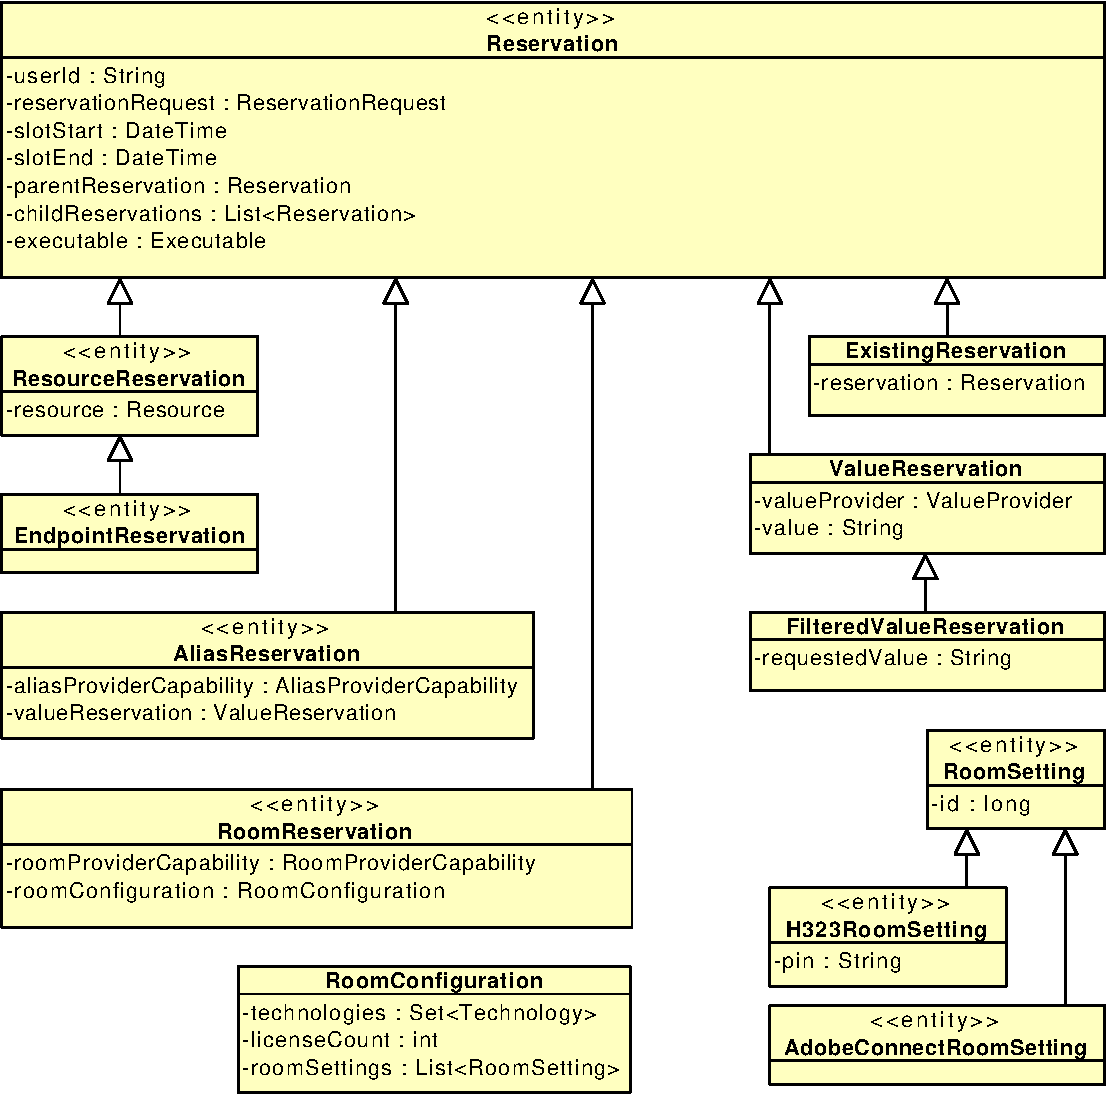
\includegraphics[width=0.7\textwidth]{diagrams/cd_reservations}
\caption{Database schema of reservations}
\label{fig:reservations}
\end{figure}



\cleardoublepage
\subsection{Executables}

\begin{figure}[ht!]
\centering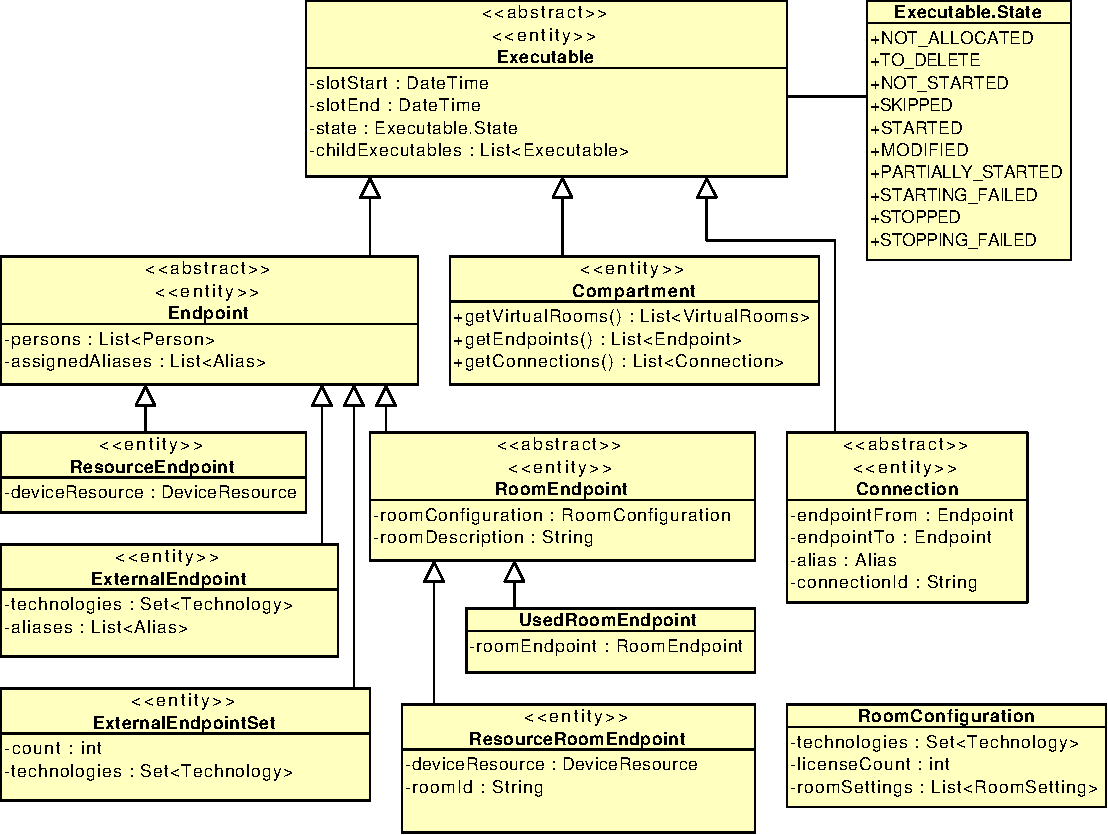
\includegraphics[width=0.8\textwidth]{diagrams/cd_executables}
\caption{Database schema of executables}
\label{fig:executables}
\end{figure}




\chapter{Web Client}

This chapter describes currently implemented web client. It allows the users to create 3 types of reservation requests:

\begin{enumerate}
\item Reservation request for (\textit{adhoc}) room in H.323/SIP MCU or meeting in Adobe Connect server for specific time slot and number of participants. 
\paragraph{Example}
\textit{An user wants to arrange a meeting for $N$ participants from 13:00 to 15:00 on 2013-04-10 and thus he creates a new request for H.323/SIP room, he gets allocated a room reservation and the room will be started exactly at 13:00 and stopped at 15:00.}

\begin{figure}[ht!]
\centering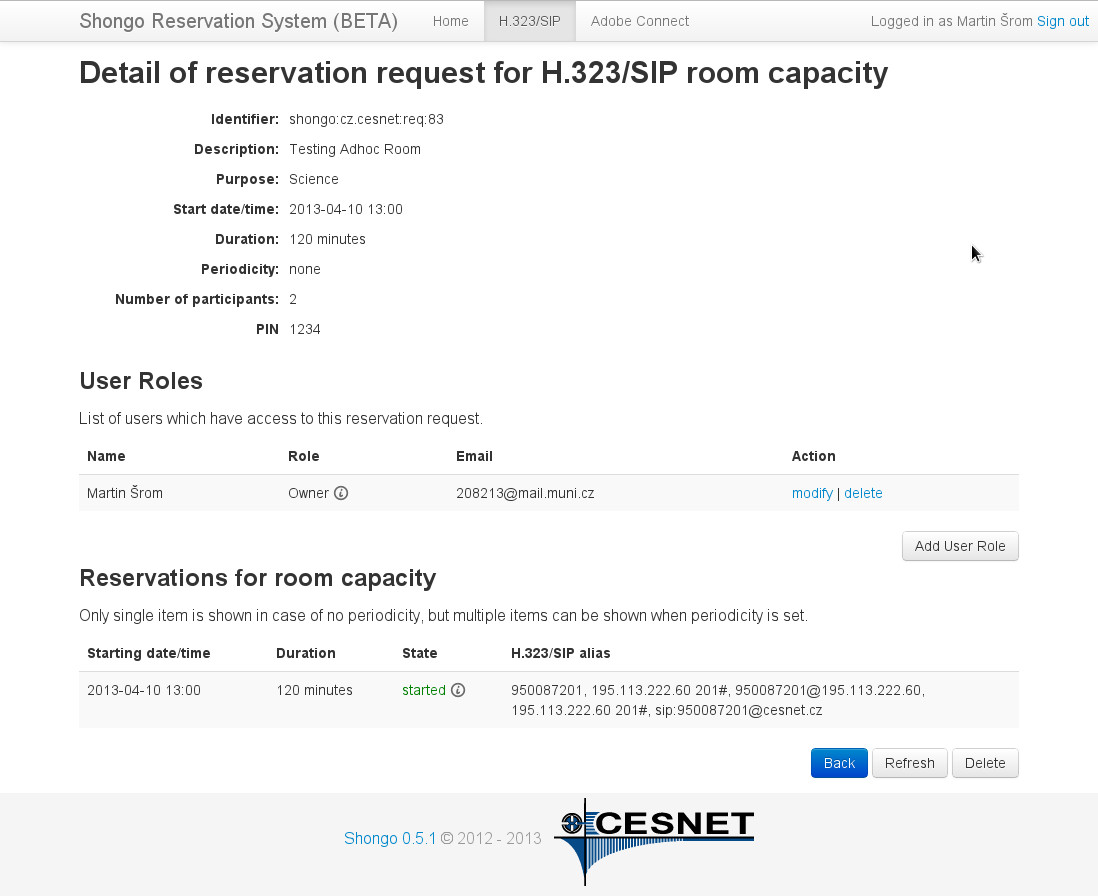
\includegraphics[width=0.7\textwidth]{images/client_web_detail_room.png}
\caption{Detail of reservation request for H.323/SIP adhoc room}
\label{fig:client-web-detail-alias}
\end{figure}

\item Reservation request for alias which then can be reused in multiple room reservation requests. Term \textit{alias} in the web client refers to the unique name of a room/meeting.

When alias for H.323/SIP MCU is allocated a room is going to be created in the target MCU with requested room name and with new allocated H.323 number.

When alias for Adobe Connect is allocated a meeting is going to be created in the target Adobe Connect server with requested room name and with URL path which is also generated from the requested room name.

By the alias reservation request the user gets a room/meeting which is created on target device for the whole requested time slot, but participants cannot join/access the room/meeting, because it is setup to consume 0 licenses in the device. To be able to join the room the user must first allocate a room capacity for the alias.

\paragraph{Example}
\textit{An user wants to have a H.323/SIP virtual room for his meetings with same name and H.323 number each time he arranges a meeting. He creates a new request for H.323/SIP alias with validity from 2013-01-01 to 2013-12-31 (in future he will be able to extend the validity). He gets allocated an alias reservation for which a room will created, but no participant will be able to join the room unless the user creates a reservation request for room capacity.}

\begin{figure}[ht!]
\centering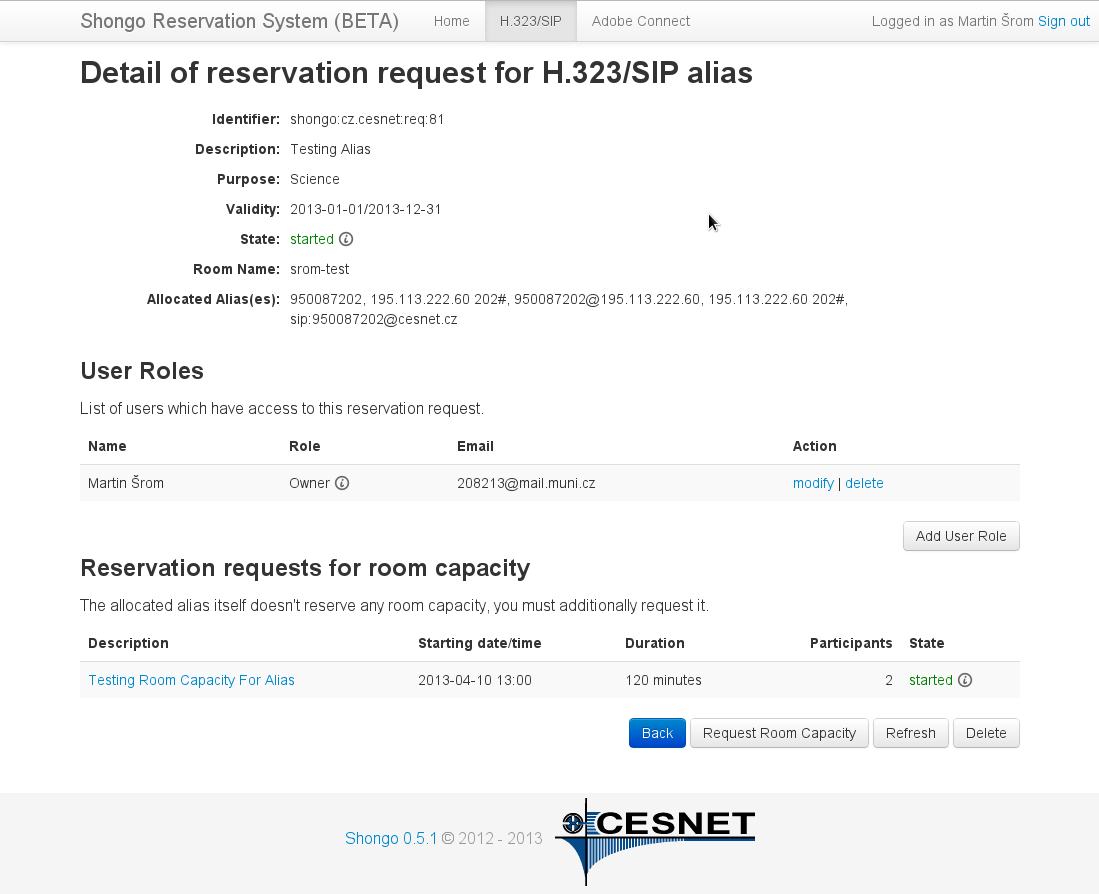
\includegraphics[width=0.6\textwidth]{images/client_web_detail_alias.png}
\parbox{10cm}{\caption{Detail of reservation request for H.323/SIP alias (unique room name \textit{srom-test} and new generated H.323 number)}}
\label{fig:client-web-detail-alias}
\end{figure}

\item Reservation request for room capacity for already allocated alias reservation request.

\paragraph{Example}
\textit{An user wants to arrange a meeting for $N$ participants from 13:00 to 15:00 on 2013-04-10 and he already has an allocated alias reservation. He creates a new request for room capacity for the alias and the room allocated by the alias will be updated according to the room capacity request from 13:00 to 15:00 ($N$ participants will be able to join the room for the time slot).}

\begin{figure}[ht!]
\centering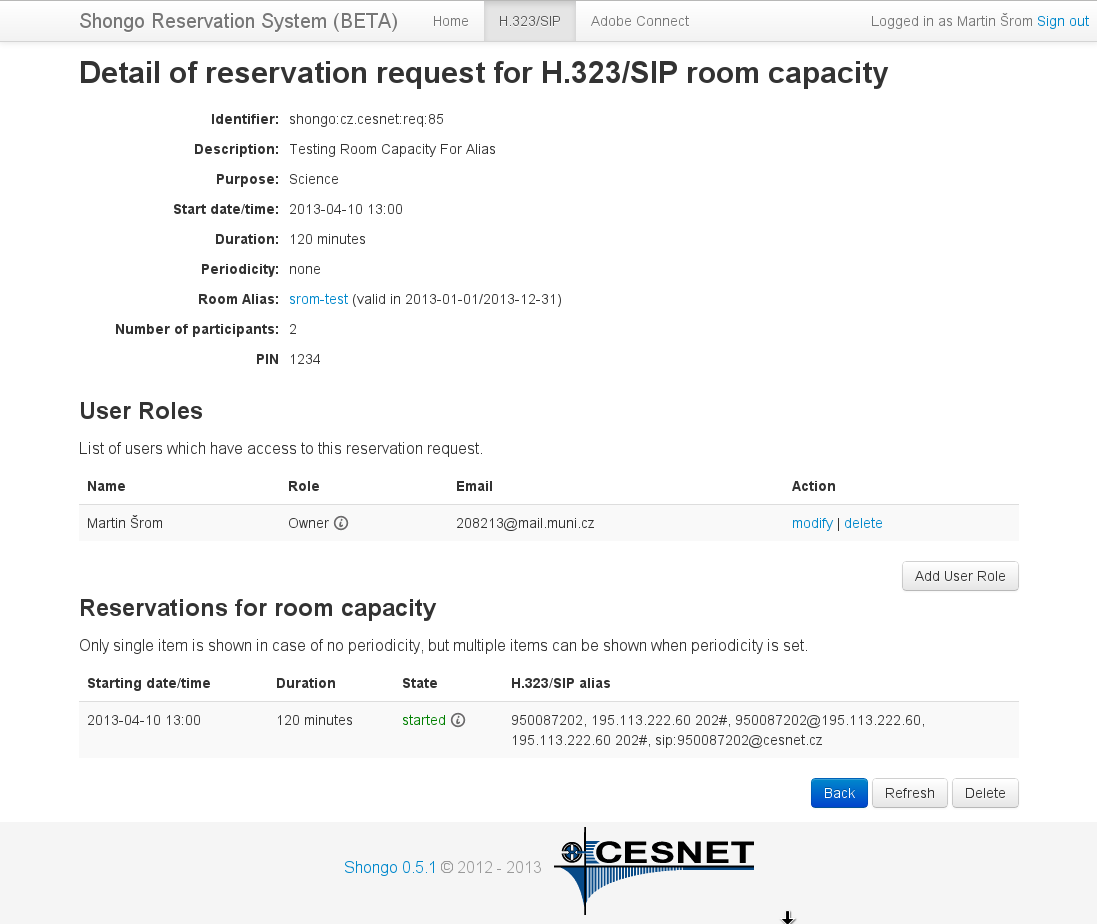
\includegraphics[width=0.6\textwidth]{images/client_web_detail_alias_room.png}
\caption{Detail of reservation request for H.323/SIP room capacity for \textit{srom-test} alias}
\label{fig:client-web-detail-alias-room}
\end{figure}

\end{enumerate}

\begin{figure}[ht!]
\centering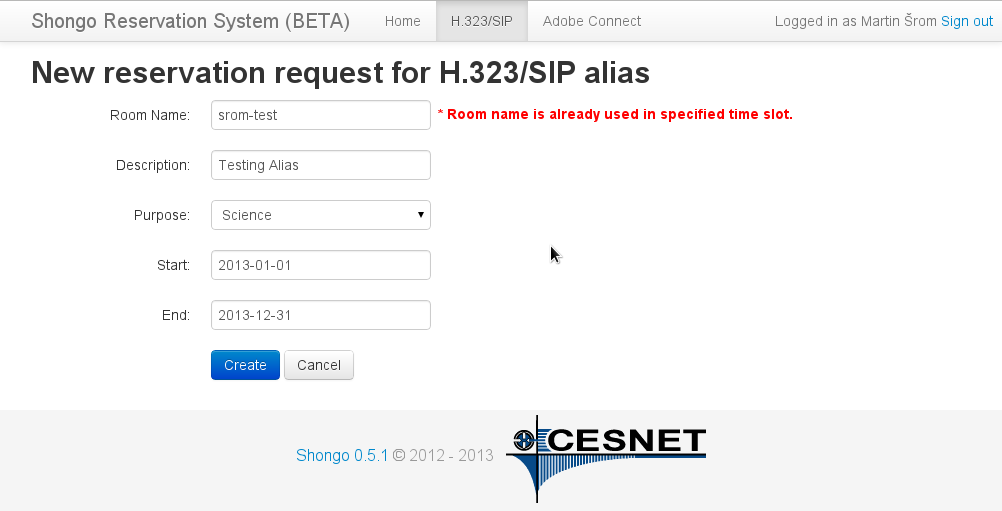
\includegraphics[width=0.6\textwidth]{images/client_web_create_alias.png}
\caption{Creating H.323/SIP alias reservation request}
\label{fig:client-web-create-alias}
\end{figure}

\begin{figure}[ht!]
\centering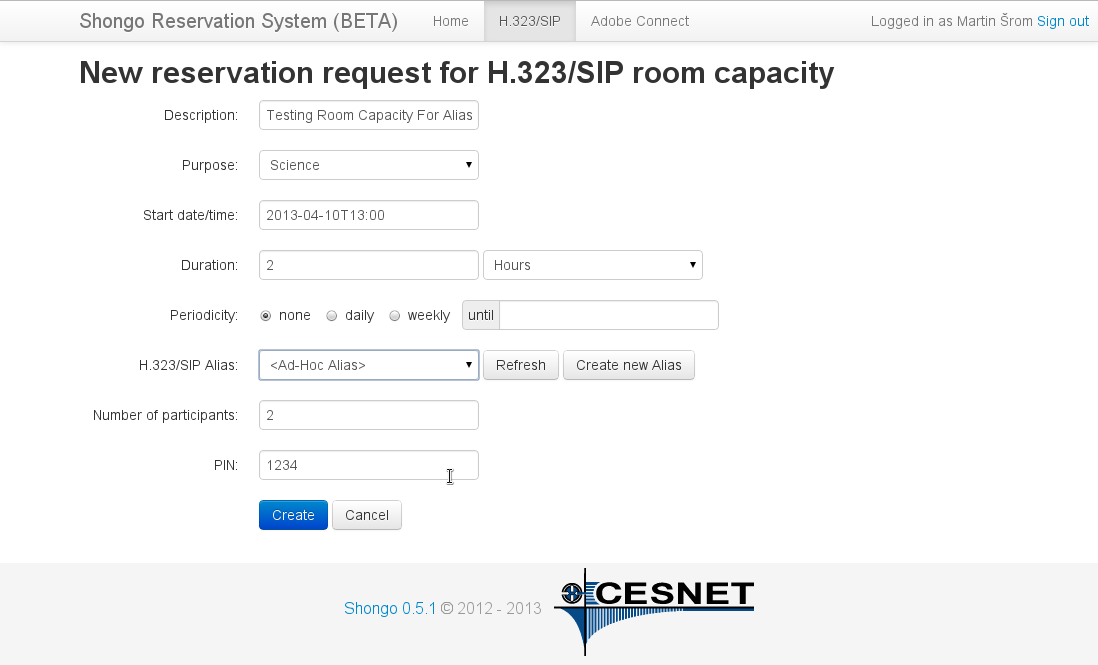
\includegraphics[width=0.6\textwidth]{images/client_web_create_room.png}
\caption{Creating H.323/SIP room reservation request}
\label{fig:client-web-create-room}
\end{figure}


\begin{figure}[ht!]
\centering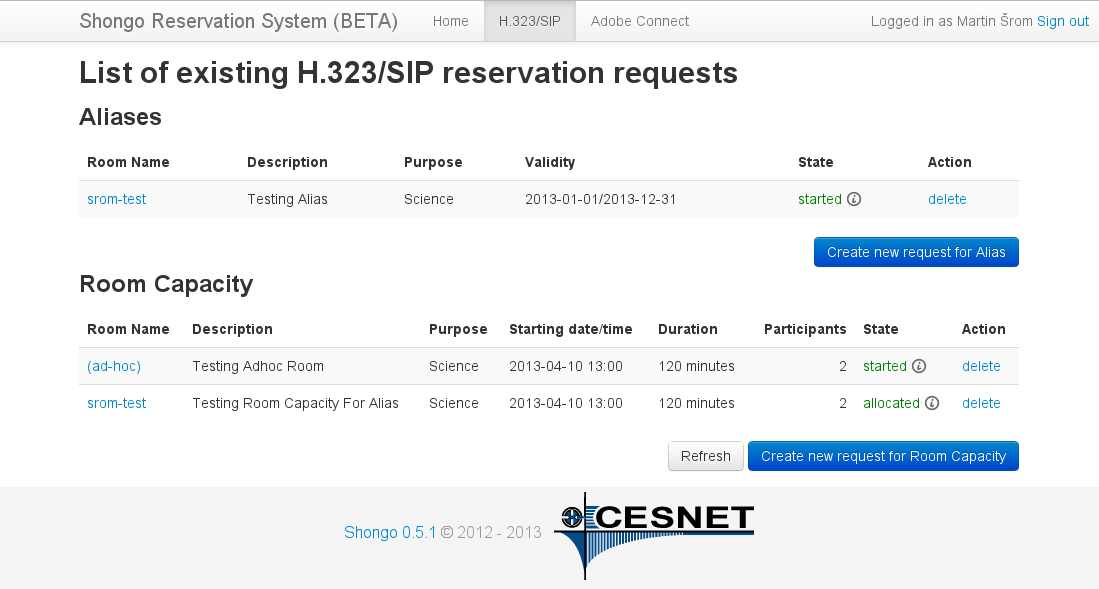
\includegraphics[width=0.6\textwidth]{images/client_web_list.png}
\caption{Main page of H.323/SIP reservation requests}
\label{fig:client-web-list}
\end{figure}




\bibliography{../bibliography}

\end{document}

